\chapter{Генерация кода из описания модели}
\label{cha:code-gen}

\section{Выбор используемой нотации}
\label{sec:notation-choice}

В качестве нотации, используемой для задания модели, выбрано подмножество языка PROMELA,
описанного в \ref{sec:promela} и используемого верификатором SPIN. Это позволяет
использовать модели, созданные для SPIN, с минимальными изменениями. 

Следующие возможности PROMELA не реализованы:

\begin{enumerate}
\item Возможность создания новых процессов (т.е. все процессы должны быть активны изначально);
\item пользовательские типы данных (структуры и перечисления);
\item синхронные каналы (т.е. каналы нулевого размера, которые представляют собой <<точки
  рандеву>> между двумя процессами); поддерживаются асинхронные каналы ненулевого размера
  (за один переход возможна только одна операция с таким каналом -- запись одним процессом
  либо чтение другим);
\item возможность обращаться к явным и скрытым (IP) переменным других процессов.
\end{enumerate}

\section{Схема процесса генерации состояний}
\label{sec:idef0-codegen}

Основное время при генерации состояний уходит на составление множества $Next(s)$ для
текущего состояний $s$. Оно заключается в вычислении условий выполнимости текущих
инструкций всех процессов, присутствующих в $s$ (отсюда мы получаем множество
незаблокированных процессов $P_{ready}(s)$), после чего для каждого процесса $P$ из
$P_{ready}(s)$ генерируется новое состояние, получающееся в результате выполнения его
текущей инструкции (номер которой хранится в $IP_P$).

Для достижения большей производительности генерация состояний осуществляется кодом на
языке~C, который, в свою очередь, генерируется из описания модели.

Процесс генерации состояний изображен на рис.~\ref{fig:idef0-codegen}. Исходное описание
модели считывается парсером и переводится во внутреннее представление в виде графа команд
и условий их выполнимости. 

% \begin{figure}[ht]
%   \centering
%   \begin{tikzpicture}[->,>=stealth',node distance=2cm]
%     \tikzstyle{state} = [circle,fill=none,draw=black,thick,text=black]
%     \tikzstyle{trans} = [rectangle split,rectangle split parts=2,rounded corners,thick,fill=none,draw=black,text=black]
%     \tikzstyle{line}  = [draw, -latex']

%     \node[state]     (S0)                     {$s_0$};
%     \node[trans]     (T0) [below       of=S0] {
%       \begin{tabular}{l}
%         \scriptsize$lfork = 0$
%         \nodepart{second}
%         \scriptsize$lfork \leftarrow 1$
%       \end{tabular}
%     };
%     \node[state]     (S1) [below       of=T0] {$s_1$};
%     \node[trans]     (T1) [below left  of=S1] {
%       \begin{tabular}{l}
%         \scriptsize$rfork = 0$
%         \nodepart{second}
%         \scriptsize$rfork \leftarrow 1$
%       \end{tabular}
%     };
%     \node[state]     (S2) [below       of=T1] {$s_2$};
%     \node[trans]     (T2) [below right of=S1] {
%       \begin{tabular}{l}
%         \scriptsize$rfork \neq 0$
%         \nodepart{second}
%         \scriptsize$lfork \leftarrow 1$
%       \end{tabular}
%     };
%     \node[state]     (S3) [below       of=T2] {$s_3$};
%     \node[trans]     (T3) [below       of=S2] {
%       \begin{tabular}{l}
%         \nodepart{second}
%         \scriptsize$n_{eat} = n_{eat} + 1$
%       \end{tabular}
%     };
%     \node[state]     (S4) [below       of=T3] {$s_4$};
%     \node[trans]     (T4) [below       of=S4] {
%       \begin{tabular}{l}
%         \nodepart{second}
%         \scriptsize$n_{eat} = n\_eat + 1$ \\
%         \scriptsize$right = 0$
%       \end{tabular}
%     };
%     \node[state]     (S5) [below       of=T4] {$s_5$};
%     \node[trans]     (T5) [below       of=S5] {
%       \begin{tabular}{l}
%         \nodepart{second}
%         \scriptsize$left = 0$
%       \end{tabular}
%     };
%     \node[state]     (S6) [below       of=T5] {$s_6$};

%     \path
%         (S0) edge (T0)
%         (T0) edge (S1)
%         (S1) edge [bend left=10] (T1)
%              edge [bend right=10] (T2)
%         (T1) edge (S2)
%         (T2) edge (S3)
%         (S2) edge (T3)
%         (T3) edge (S4)
%         (S4) edge (T4)
%         (T4) edge (S5)
%         (S5) edge (T5)
%         (T5) edge (S6)
%         (S6) edge [bend left=50] (S0)
%         (S3) edge [bend right=50] (S0);
%   \end{tikzpicture}
%   \caption{Пример}
%   \label{fig:inner-graph}
% \end{figure}

!!! пример !!!

!!! use case !!! 

\begin{figure}[ht]
  \centering
  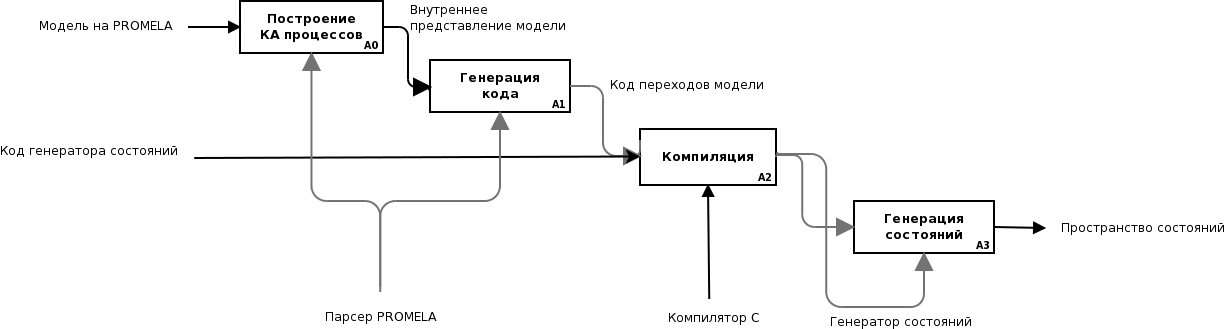
\includegraphics[width=1\textwidth]{../../graphics/idef0-codegen}  
  \caption{Схема процесса верификации}
\label{fig:idef0-codegen}
\end{figure}

Генерируемый код на~C проверяет условия выполнимости текущих инструкций всех процессов и,
в случае выполнимости процесса $P$, создает новое состояние, являющееся копией текущего, и
модифирует его в соответствии с текущей инструкцией $P$.

Таким образом, генерируются следующие части кода:

\begin{itemize}
\item проверка выполнимости процессов данного состояний;
\item модификация состояния в соответствии с текущей инструкцией данного процесса;
\item вспомогательный код (отладочная печать состояния и т.п.).
\end{itemize}

Полученный код компилируется и компонуется вместе вместе с программой-<<драйвером>>
(осуществляющей выполнение не зависящих от конкретной модели операций: хэширование и
хранение состояний, передача по сети и~т.д.). Программа-<<драйвер>> делает вызовы функций
сгенерированного кода для вычисления $Next(s)$.

<<Драйверов>> имеется два: 

\begin{itemize}
\item последовательный, использованный в \ref{cha:paremu} для имитации параллельного
  выполнения с целью оценки распредления состояний;
\item описанный в \ref{cha:parmpi} параллельный на MPI.
\end{itemize}

\section{Генератор кода}
\label{sec:promela-parser}

Парсер описания модели и генератор кода написан на языке Python. В качестве парсера
используется штатный GLR-парсер \Code{Pyggy}. Диаграмма классов генератора показана на
рис.~\ref{fig:pmlparse-classes}.

\begin{figure}[ht]
  \centering
  \includegraphics[width=1\textwidth]{../../graphics/pmlparse-classes}
  \caption{Диаграмма классов генератора кода}
  \label{fig:pmlparse-classes}
\end{figure}

%%% Local Variables: 
%%% mode: latex
%%% TeX-master: "main"
%%% End: 
